\documentclass[runningheads]{llncs} % template "Lecture notes for computer science"
\usepackage[spanish]{babel} % para el texto en espanhol
\usepackage{graphicx} % para imaganes
\graphicspath{{images/}} % ruta a la carpta de imagenes
\usepackage{hyperref} % para los hipervinculos
\usepackage{xurl} % para el line braker de los url
\usepackage{xcolor} % para definir colores custom
% \definecolor{royalblue(web)}{rgb}{0.25, 0.41, 0.88}
% \definecolor{royalblue(traditional)}{rgb}{0.0, 0.14, 0.4} no funca
\hypersetup{ % configuracion de los hiper vinculos
    colorlinks=true,
    linkcolor=black,
    filecolor=black,      
    urlcolor=blue,
    citecolor=black, % ver si poner en blue o dejar asi
    pdftitle={Redes neuronales},
    pdfpagemode=FullScreen,
}
\usepackage[T1]{fontenc} % para la codificacion de la fuente.
\usepackage[backend=biber,style=numeric]{biblatex} % para la bibliografia.
\addbibresource{bibliografia.bib} % incluir el .bib
\usepackage{csquotes} % para que los textos citados esten con tipografia de acuerdo con las reglas de csquotes
% \usepackage{amssymb} % simbolos matematicos
\usepackage{amsmath}

\begin{document}

% =================================================================================
% PORTADA
% =================================================================================
\title{Redes neuronales y sus aplicaciones recientes}

%\titlerunning{Abbreviated paper title}
% If the paper title is too long for the running head, you can set
% an abbreviated paper title here
%
\author{Alain Vega \\ \email{alainjosevz@gmail.com}}
%
\authorrunning{Alain Vega}
% First names are abbreviated in the running head.
% If there are more than two authors, 'et al.' is used.
%
\institute{Universidad Catolica "Nuestra señora de la Asuncion" \\ 
Facultad de ciencias y tecnologia \\
Departamento de electronica e informatica \\
\url{https://www.universidadcatolica.edu.py/} }
%
\maketitle              % typeset the header of the contribution
%
\begin{abstract}
Una de las tendencias ultimamente son las redes neuronales. En este documento
se muestran conceptos claves sobre este modelo y una significativa variedad
de ejemplos sobre aplicaciones recientes del mismo.

\keywords{Redes neuronales \and Inteligencia artificial \and Aprendizaje automatico
\and Aprendizaje profundo. \and Neural networks \and Artificial inteligence 
\and Machine learning \and Deep learning \and AI \and ML \and NN \and ANN 
\and SNN \and DL}
\end{abstract}
% =================================================================================
% CONTENIDO
% =================================================================================
\section{Introduccion}
Si hace unos años, nos hubieran dicho que una máquina sería capaz de aprender 
por sí sola y tomar decisiones basadas en esa experiencia, ¿te lo habrías creído? 
¿Y si además te hubieran dicho que un conjunto de algoritmos serían capaces de
hacer funciones consideradas \textquotedblleft{humanas}\textquotedblright{}
como crear arte o componer melodías únicas? \cite{int1}

Todo esto es ya una realidad, por ello ultimamente la Inteligencia artificial (AI) 
esta en boca de todos, pero es gracias a las \textbf{redes neuronales} (NN)
que todo esto es posible. 

Estas redes alcanzan metas bastante impresionantes y que cada vez se acercan 
más a esa idea original de reproducir el funcionamiento del cerebro humano 
en una computadora. 

Ahora bien, ¿en qué consisten estos modelos? ¿Cómo puede imitar un computadora 
el proceso de aprendizaje y acabar desarrollando una
\textquotedblleft{cosa}\textquotedblright{} que funciona? \cite{int2}
\section{¿Que es una red neuronal?}
Una red neuronal, tambien conocida como red neuronal artificial (ANN)
o red neuronal simulada (SNN), es un modelo de \textit{machine learning} (ML)
el cual constituye el eje de los algoritmos de \textit{deep learning} (DL) 

Su nombre y estructura se inspiran en el cerebro humano, 
e imitan la forma en la que las neuronas biológicas se señalan entre sí.

Las redes neuronales artificiales (ANN) están formadas por capas de nodos, 
que contienen una capa de entrada, una o varias capas ocultas y una capa de salida.
\cite{def-ibm1}

Donde cada nodo se conoce como una neurona artificial, esta se conecta a 
otra neurona (nodo) la capa hace referencia a conjunto de nodos (neuronas).

\begin{figure}
    \centering
    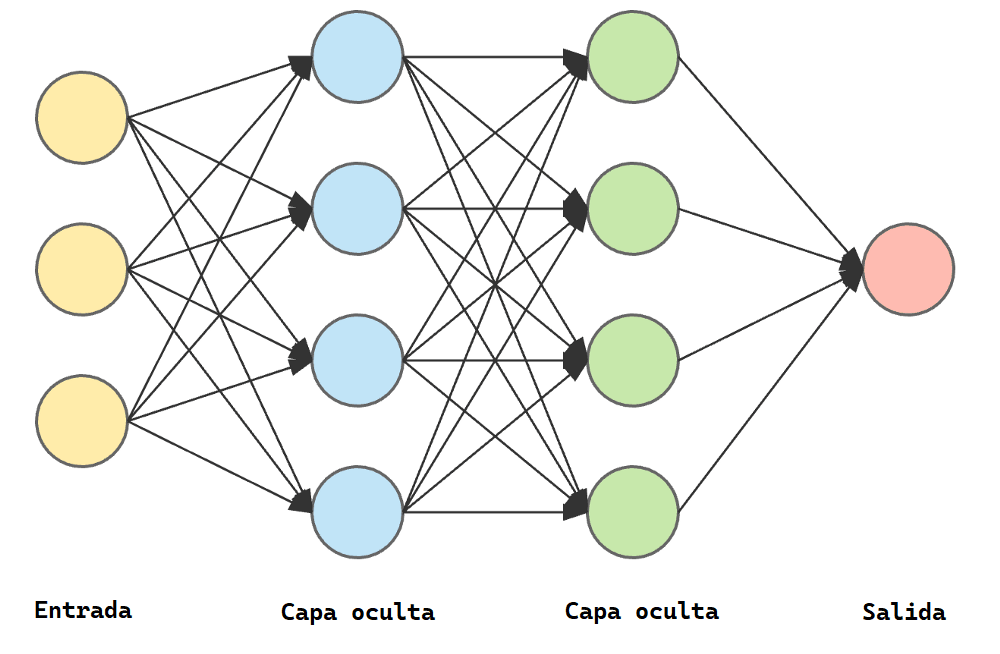
\includegraphics[scale=0.6]{red_neuronal_artificial.png}
    \caption{Ejemplo de una red neuronal artificial (ANN) \cite{int1}}
    \label{fig:red_neuronal_artificial}
\end{figure}

En la figura \ref{fig:red_neuronal_artificial} se muestra un ejemplo,
aqui la capa de la izquierda es la capa de entrada (la que esta
conectada con el \textquotedblleft{mundo}\textquotedblright{} exterior y se alimenta de el)
las capas 2 y 3 son capas ocultas que ayudan al procesamiento
de la tarea y por ultimo la capa 4 es la de salida, la cual
envia sus resultados al \textquotedblleft{mundo}\textquotedblright{} exterior

\section{Estructura basica de una red neuronal}
\subsection{Analogia con el cerebro}
La neurona es la unidad fundamental del sistema nervioso y en particular 
del cerebro. Cada neurona es una simple unidad procesadora que recibe y combina 
señales desde y hacia otras neuronas. 
Si la combinación de entradas es suficientemente fuerte la salida de la neurona
se activa. \cite{libro-def}

\begin{figure}
    \centering
    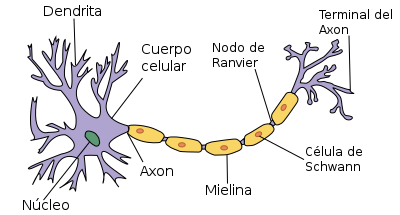
\includegraphics[scale=0.7]{neurona_real.png}
    \caption{Componentes de una reurona real \cite{img-neurona_real}}
    \label{fig:neurona_real}
\end{figure}

El cerebro consiste en uno o varios billones de neuronas densamente 
interconectadas. Apoyandonos en la figura \ref{fig:neurona_real}.
El axón (salida) de la neurona se ramifica y está conectada a las dendritas (entradas) 
de otras neuronas a través de uniones llamadas sinapsis.
La eficacia de la sinpasis es modificable durante el proceso de 
aprendizaje de la red. \cite{libro-def}

\subsection{Redes neuronales artificiales (ANN)}
En las Redes Neuronales Artificiales, ANN, la unidad análoga a la neurona biológica es
el elemento procesador, PE (\textit{Process Element}). Un elemento procesador tiene varias
entradas y las combina, normalmente con una suma básica. 
\footnote[1]{Existen mas formas de combinar las entradas de la neurona 
que la sumatoria, como por ejemplo con un productorio: \(\Pi_{i}{w_{i}*x_{i}}\)
o aplicando la funcion maximo elemento: \(\max_{i}{w_{i}*x_{i}}\) \cite{tesis-matich}}.
La suma de las entradas es
modificada por una función de transferencia y el valor de la salida de esta función de
transferencia se pasa directamente a la salida del elemento procesador.
\footnote[2]{En lugar de pasar el valor de la funcion de transferencia
directamente a la salida (funcion de salida = funcion identidad), 
se puede pasar por otra funcion, \textbf{la funcion de salida} 
la cual pueder ser una funcion binaria \cite{tesis-matich} \\
\(B(x)=1\) si \(x>=umbral\), \\
\(B(x)=0\) caso contario}

La salida del PE se puede conectar a las entradas de otras neuronas artificiales (PE)
mediante conexiones ponderadas correspondientes a la eficacia de la sinapsis de las
conexiones neuronales. \cite{libro-def}

\begin{figure}
    \centering
    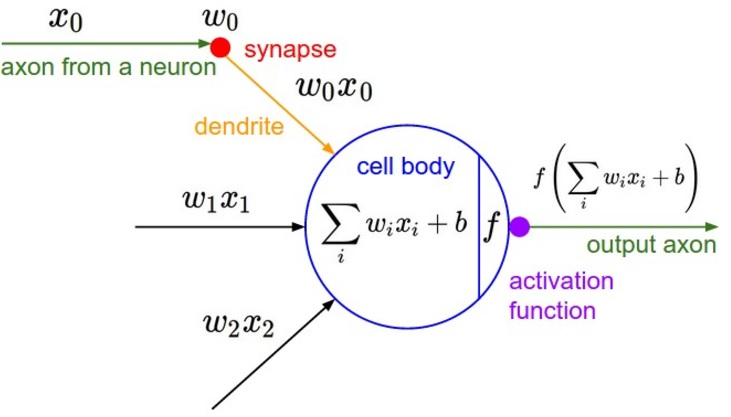
\includegraphics[scale=0.7]{neurona_artificial2.png}
    \caption{Diagrama de una neurona artificial con conceptos de una neurona real \cite{img-neurona_artificial2}}
    \label{fig:neurona_artificial}
\end{figure}

La Figura \ref{fig:neurona_artificial} muestra una neurona artificial con conceptos
de una neurona real.
La dendrita se representa como un enlace de entrada a la neurona.

La sinapsis se representa como la union/fusion de un terminal del axon de una neurona
con una dendrita de otra neurona. 

En el cuerpo celular ocurren varias cosas, la primera es que gracias a sinapsis las
entradas disponibles de cada una de las neuronas de la capa anterior llegan como el 
producto \(x_{i}*w_{i}\), donde \(x_{i}\) es el resultado de una neurona 
\textquotedblleft{anterior}\textquotedblright{} y \(w_{i}\) es el peso 
\textquotedblleft{conectarse}\textquotedblright{} a la dendrita de nuestra neurona.
La segunda es la sumatoria de cada entradas \(x_{i}*w_{i}\) y sumarle
\(b\) que representa el bias/sesgo/umbral (el cual nos permite mover la funcion
de activacion de manera horizontal).
Por ulitmo toda la sumatoria del paso dos, se pasa a la funcion de activacion \(f\)
esta puede lineal o no lineal, existen una amplia variedad de funciones de activacion.

Finalmente transmite el resultado \(y = f(\sum_{i=1}^{n}{x_{i}*w_{i}} + b)\)
suponiendo \textit{n} entradas

\section{Funcion de activacion}
La funcion de activacion se encarga de decidir cuando una neurona artificial debe activarse
o no. Esto significa que dicha funcion decide cuando la entrada a la neurona artificial
es importante o no para la red. \cite{fun-activacion}

Su rol es derivar la salida de la neurona artificial, dado un conjunto de valores de la entrada
para alimentar a otras neuronas artificiales. \cite{fun-activacion}

Existen muchas funciones de activacion, se pueden clasificar en tres grupos.
\subsection{Clases de funciones de activacion}

\subsubsection{Funciones de paso binario}
Necesita de un valor umbral \(\xi\) que decide cuando la neurona artificial debe activarse o no.
\cite{fun-activacion}

\[
    B(x) =
    \left \{
        \begin{aligned}
        0, \ \ & \text{si } x < \xi  \\
        1, \ \ & \text{si } x \geq \xi
        \end{aligned}
    \right .
\]


% Por motivos de simplicidad desde este punto hasta el final del documento, 
% cada vez que aparezca la frase \textquotedblleft{red neuronal}\textquotedblright{} y 
% \textquotedblleft{neuronal}\textquotedblright{}
% se hace referencia a la \textquotedblleft{red neuronal artificial}\textquotedblright{} y 
% a la \textquotedblleft{neuronal artificial}\textquotedblright{} respectivamente,
% se precisara cuando se hable de una neurona real.

\subsubsection{Funciones de activacion lineales}
Tambien conocida como \textquotedblleft{}sin activacion\textquotedblright{} 
donde la activacion es proporcional a la entrada. \cite{fun-activacion2} \\
Se utilizan en la capa de salida para problemas de regresion lineal. \cite{fun-activacion}

\[ f(x)=mx+b \]

\subsubsection{Funciones de activacion no lineales}
Son las mas utilizadas ya que facilita que el modelo generice o se adapte con una 
variedad de datos y diferencie entre los resultados. \cite{fun-activacion2}

Las principales son: 
\begin{itemize}
    \item{\textbf{Sigmoide o logistica}: utlizada en la capa de salida
    para problemas de clasificacion binaria (clasificar en 2 grupos) y problemas
    de clasificacion multietiqueta o multi-objetivo (la salida puede estar 
    en mas de un grupo). \cite{fun-activacion}
    \[\sigma(x) = \frac{1}{1-e^{-x}}\] } 
    \item{\textbf{Tangente hiperbolico}: utilizada en las capas ocultas 
    de una red neuronal recurrent (RNN). \cite{fun-activacion}
    \[\tanh(x) = \frac{e^{x}-e^{-x}}{e^{x}+e^{-x}}\]}
    \item{\textbf{ReLU (\textit{Rectified Linear Unit})}: utilizada en las capas
    ocultas de una red neuronal convolucional (CNN). \cite{fun-activacion}
    \[ReLU(x) = max(0,x)\]} 
    \item{\textbf{Softmax}: utilizada en la capa de salida para problemas
    de multi-clasificacion (clasificar en mas de 2 grupos). \cite{fun-activacion}
    \[ s(x_{i}) = \frac{e^{x_{i}}}{\sum_{j=1}^{n}{e^{x_{j}}}} \]}\\
    La funcion Softmax convierte el vector de \textit{K} entradas a un vector 
    de \textit{K} salidas tal que la suma las salidas es igual a 1,
    entonces la salida se puede interpretar como una distribucion de probabilidades.
    \cite{fun-softmax}
\end{itemize}

\subsection{Tipos de Redes neuronales}
\subsection{AI vs ML vs NN vs DL}
\section{Conocimiento}
\subsection{¿Como aprenden estas redes?}
\subsubsection{Propagacion hacia atras}
\subsection{¿Representa como aprendemos los humanos?}
\section{Aplicaciones}
\subsection{Ejemplo1}
\subsection{Ejemplo2}
\subsection{Ejemplo3}
\subsection{Ejemplo4}
\subsection{Ejemplo5}
\section{Conclusion}

\newpage
\printbibliography

\end{document}